\documentclass[12pt,twoside]{article}

\newcommand{\reporttitle}{M111: Big Data Management}
\newcommand{\reportauthor}{Michael Darmanis\textsuperscript{*}}
\newcommand{\reporttype}{Project}
\newcommand{\sid}{7115152200004}

% include files that load packages and define macros
\input{includes} % various packages needed for maths etc.
\input{notation} % short-hand notation and macros


%%%%%%%%%%%%%%%%%%%%%%%%%%%%

\begin{document}
% front page
% Last modification: 2016-09-29 (Marc Deisenroth)
\begin{titlepage}

\newcommand{\HRule}{\rule{\linewidth}{0.5mm}} % Defines a new command for the horizontal lines, change thickness here


%----------------------------------------------------------------------------------------
%	LOGO SECTION
%----------------------------------------------------------------------------------------

\includegraphics[width=7cm]{./figures/NKUA-logo}\\[0.5cm]

\begin{center} % Center remainder of the page

%----------------------------------------------------------------------------------------
%	HEADING SECTIONS
%----------------------------------------------------------------------------------------
\textsc{\LARGE \reporttype}\\[1.5cm] 
\textsc{\Large National and Kapodistrian University of Athens}\\[0.5cm] 
\textsc{\large Faculty of Informatics and Telecommunications }\\[0.5cm]
% \textsc{\large MSc. Data Science and Information Technologies}\\[0.5cm]
%----------------------------------------------------------------------------------------
%	TITLE SECTION
%----------------------------------------------------------------------------------------

\HRule \\[0.4cm]
{ \huge \bfseries \reporttitle}\\ % Title of your document
\HRule \\[1.5cm]
\end{center}
%----------------------------------------------------------------------------------------
%	AUTHOR SECTION
%----------------------------------------------------------------------------------------

%\begin{minipage}{0.4\hsize}
\begin{flushleft} \large
\textit{Author:}\\
\reportauthor~(SID: \sid)% Your name
\end{flushleft}
\vspace{2cm}
\makeatletter
Date: \@date\\
\textsuperscript{*}\href{mailto:mdarm@di.uoa.gr}{mdarm@di.uoa.gr}

\vfill % Fill the rest of the page with whitespace



\makeatother


\end{titlepage}



%%%%%%%%%%%%%%%%%%%%%%%%%%%% Main document
\section*{Introduction}

The following representation provides a structured overview of the project's directory hierarchy, and can serve as a quick reference to the deliverables and components. This layout details the various output files, source code modules and the report itself.

\begin{minted}[breaklines, breakafter=d]{bash}
$PROJECT_ROOT
¦   # Project's outputs
+-- output
¦   ¦   # Execution times with and without the optimiser
¦   +-- catalyst_times.txt
¦   ¦   # Query outputs using the RDD API
¦   +-- df_results
¦   ¦   ¦
¦   ¦   +-- Q1DF.txt
¦   ¦   +-- Q2DF.txt
¦   ¦   +-- Q3DF.txt
¦   ¦   +-- Q4DF.txt
¦   ¦   +-- Q5DF.txt
¦   ¦
¦   +-- join_outputs.txt        # outputs when using broadcast and repartition joins
¦   +-- join_type_times.txt     # execution times when using broadcast and repartition joins
¦   +-- non_optimised_plan.txt  # quey plan without using Catalyst
¦   +-- optimised_plan.txt      # query plan with Catalyst
¦   +-- part_1_times.txt        # execution times, for every query, for all data types
¦   +-- coursework.pdf          # project's report
¦   ¦   # Query outputs using the Dataframe API
¦   +-- rdd_results
¦       ¦
¦       +-- Q1RDD.txt
¦       +-- Q2RDD.txt
¦       +-- Q3RDD.txt
¦       +-- Q4RDD.txt
¦       +-- Q5RDD.txt
¦   # Modules for performing all tasks
+-- src
    ¦
    +-- csv_to_parquet.py       # converting the csv files to parquet
    +-- joins.py                # performing broadcast and repartition joins
    +-- main.py                 # running script; executes required tasks
    +-- optimiser.py            # enabling and disabling Catalyst
    +-- rdd.py                  # rdd queries
    +-- sql_csv.py              # csv queris (SQL-like)
    +-- sql_parquet.py          # parquet queries (SQL-like)
    +-- utils.py                # helper functions
\end{minted}

All of the code (modules in the \texttt{src} files) is also included in Part~\ref{snippets}, at the end of this document. Note that because of Java heap errors, the following modification was made in the \texttt{spark-defaults.conf} file:
\mint{bash}|spark.driver.memory 1024m|

\section{File Management in HDFS}
\subsection{Save files in HDFS}
For creating a \texttt{files} directory in the HDFS, the following command was used
\mint{bash}|hadoop fs -mkdir -p ~/files|
\noindent and to populate it with the project's \texttt{.csv} files
\mint{bash}|hadoop fs -put *.csv ~/files .|
\noindent Since the only \texttt{.csv} files populating the working directory were the project's ones, it was fairly easy to fetch all of them using \texttt{*.csv}.

Figure~\ref{fig:files} shows a print-screen of the \texttt{.csv} files lying within the created \texttt{files} directory.

\begin{figure}[htbp]
    \centering
    \includegraphics[width=\textwidth]{./figures/files.png}
    \caption{HDFS directory containing the project's datasets in \texttt{.csv} format.}
    \label{fig:files}
\end{figure}

The same files were then saved in \texttt{.parquet} format, using Snippet~\ref{code:files}, as can be seen in the print-screen of Figure~\ref{fig:files-all}.

\begin{figure}[htbp]
    \centering
    \includegraphics[width=\textwidth]{./figures/files-all.png}
    \caption{HDFS directory containing the project's datasets in both \texttt{.csv} and \texttt{.parquet} formats.}
    \label{fig:files-all}
\end{figure}

\subsection{RDD queries}
All of the RDD queries can be found in the \texttt{rdd.py} module (see Snippet~\ref{code:rdd}). All performed joins, when required, were repartition joins. Below is the execution of query 1: ``Get the difference betwen revenue and production cost (i.e. profits) of every movie after 1995.'' 

\inputminted[breaklines, breakafter=d, linenos, firstline=18, lastline=24]{python}{./code/rdd.py}

\subsection{Dataframe queries}
All of the Dataframe queries can be found in the \texttt{sql\textunderscore csv.py} and \texttt{sql\textunderscore parquet.py} modules (see Snippets~\ref{code:sql-csv}~\&~\ref{code:sql-parquet}). Below is the execution of query 1: ``Get the difference betwen revenue and production cost (i.e. profits) of every movie after 1995.''

\inputminted[breaklines, breakafter=d, linenos, firstline=59, lastline=65]{python}{./code/sql_csv.py}

\subsection{Query execution-times}

To ensure the highest precision in measurement-performance, a Spark benchmarking approach was used. For each individual case, a distinct Spark session was instantiated, and after the run, was terminated. This strategy was imperative to prevent data or intermediate computations from being cached, thereby eliminating any potential biases. This guarantees that the analysis is grounded in somewhat representative query execution-times. The results can be seen in Figure~\ref{fig:execution-times}.

\begin{figure}[!htbp]
    \centering
    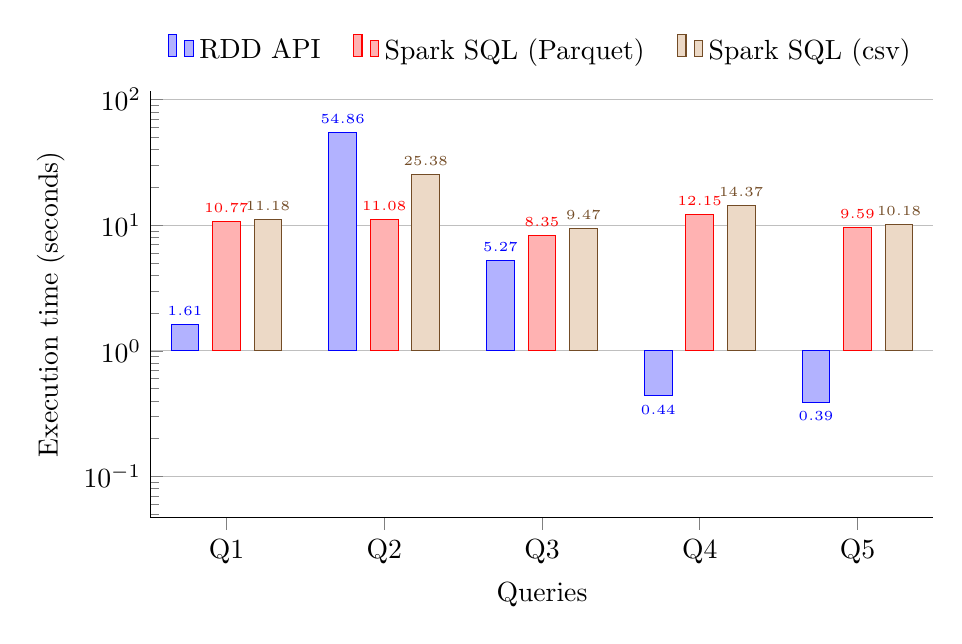
\begin{tikzpicture}
\begin{axis}[
    ybar=5pt,
    enlargelimits=0.12,
    bar width=10pt,
    ylabel={Execution time (seconds)},
    xlabel={Queries},
    width=0.95\textwidth,
    height=7cm,
    symbolic x coords={Q1,Q2,Q3,Q4,Q5},
    xtick=data,
    ymode=log,
    ymin=0.1,
    ymajorgrids=true,
    axis x line* = bottom,
    axis y line* = left,
    legend style={cells={anchor=west}, draw=none},
    legend style={at={(0.5,1.15)}, anchor=north,legend columns=-1},
    legend columns=-1,
    point meta=explicit symbolic,
    nodes near coords=\pgfmathprintnumber{\pgfplotspointmeta},
    visualization depends on={y<0.2?0:1 \as \myshift},
    every node near coord/.append style={font=\tiny, anchor=north, yshift=(\myshift*10pt)},
    ]
\addplot table [meta=Y] {
  X Y
  Q1  1.61
  Q2 54.86
  Q3  5.27
  Q4  0.44
  Q5  0.39
};

\addplot table [meta=Y] {
  X Y
  Q1 10.77
  Q2 11.08
  Q3  8.35
  Q4 12.15
  Q5  9.59
};

\addplot table [meta=Y] {
  X Y
  Q1 11.18
  Q2 25.38
  Q3  9.47
  Q4 14.37
  Q5 10.18
};

\legend{RDD API\hphantom{xz}, Spark SQL (Parquet)\hphantom{xz} , Spark SQL (csv) }
\end{axis}
\end{tikzpicture}
    \caption{Query execution-times, for all queries, using RDDs, CSVs and Parquet.}
    \label{fig:execution-times}
\end{figure}

A first look at the results reveals contrasting execution times with regards to the RDDs. \textit{Query 1} was completed in a mere 1.55 seconds, while \textit{queries 4 and 5} in under 1 second. On the other hand, \textit{query 2} lasted 57.27 seconds. This variance can largely be traced back to the nature of the operations and transformations inherent to each query. \textit{Query 2} was largely defined by multiple transformations (like `map', `filter', `union', `flatMap' etc.) and complex computations (like `reduceByKey' and `groupByKey') involving shuffling, which is time-intensive.
 
Furthermore, CSV files must either infer the schema or have it explicitly provided. This schema management can introduce overhead. This is exacerbated for large data sets or complex schema structures. To illustrate: \textit{query 2} took 19.66 seconds, significantly faster than its Parquet counterpart. This behaviour is expected given the inherent row-based orientation of CSVs, which is sub-optimal for Spark's preferred columnar computations. However, in \textit{queries 3, 4 \& 5}, all operations on CSV files outperformed their Parquet counterparts.

Even though Parquet often delivers commendable performance, it's crucial to note that, under situations with limited columnar data operations, or when full-file scans are inevitable, Parquet's performance can fall behind that of CSVs due to the overhead from decompressing and decoding columnar data. A very likely scenario for \textit{queries 3, 4 \& 5}.

\section{Optimised Join Strategies}
\subsection{Repartition and Broadcast Joins}
 This part focused on joining two relations, `departments' and `employees', on the `department id' attribute. While there are multiple strategies to do this, two distinct approaches were implemented: the Repartition Join and the Broadcast Join. These operations not only illustrate the diversity in handling data merges but also emphasise the significance of choosing an optimised strategy based on data size and structure. The execution of these joins can be found within the \texttt{joins.py} module (see Snippet~\ref{code:joins}).

\subsubsection{Repartition join}
This method represents a co-grouping-based join operation. The records from each RDD are tagged with their respective source labels (`employees' or `departments'). By unionising these tagged RDDs, and grouping by their keys, a co-group operation is achieved. After this, the join operation is performed by matching keys, yielding combined records from both employees and departments.

\inputminted[breaklines, breakafter=d, linenos, firstline=11, lastline=39]{python}{./code/joins.py}

\subsubsection{Broadcast join}

In this approach, the join operation leverages Spark's broadcasting capability. A dictionary (or lookup map) is created for the `departments' RDD. This dictionary gets broadcast across the cluster, enabling each node to access it locally. The join is then executed by mapping over the `employees' RDD and fetching the corresponding department name from the broadcasted dictionary using the department ID. This technique benefits from reduced data shuffling, particularly when one of the datasets (like `departments') is considerably smaller than the other.

\inputminted[breaklines, breakafter=d, linenos, firstline=42, lastline=71]{python}{./code/joins.py}

\subsection{Tweaking the Catalyst Optimiser}

Running a query with, and without, the Catalyst optimiser is performed in the \texttt{optimiser.py} module (see Snippet~\ref{code:optimiser}). Figure~\ref{fig:optimiser} shows the execution times for the following query:

\begin{minted}[breaklines, breakafter=d]{sql}
query = """
        SELECT *
        FROM (SELECT * FROM genres LIMIT 100) AS g, ratings AS r
        WHERE r.mv_id = g.mv_id
"""
\end{minted}

\begin{figure}[htb]
    \centering
    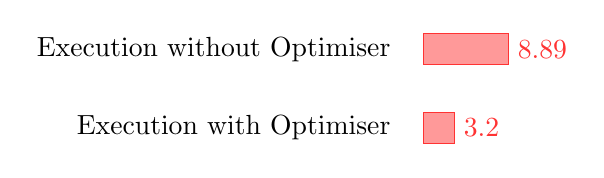
\begin{tikzpicture}
  \begin{axis}[,
    xbar,
    y axis line style = { opacity = 0 },
    axis x line       = none,
    tickwidth         = 0pt,
    ytick             = data,
    enlarge y limits  = 0.2,
    enlarge x limits  = 1,
    y = 1cm,
    width=0.3\textwidth,
    bar width=4mm,
    symbolic y coords = {Execution with Optimiser, Execution without Optimiser},
    nodes near coords,
  ]
  \addplot[red!80, fill=red!40] coordinates { (3.20,Execution with Optimiser) (8.89,Execution without Optimiser)};
  \end{axis}
\end{tikzpicture}
    \caption{Execution time, for the aforementioned query, with and without Spark's Catalyst Optimiser.}
    \label{fig:optimiser}
\end{figure}

The full query-plans, for using and without using Catalyst, can be found at the \texttt{optimised\textunderscore plan.txt} and \texttt{non\textunderscore optimised\textunderscore plan.txt} files respectively.

\subsubsection{Without Catalyst (Sort Merge Join)}

\begin{minted}{bash}
== Physical Plan ==
*(6) SortMergeJoin [mv_id#8], [mv_id#1], Inner
\end{minted}

When not using Catalyst, a Sort Merge Join is opted. This is a process where two dataframes are merged post-sorting. Such joins are prevalent when data cannot fit into memory for a Broadcast Join (this is a fallacious statement in this case of course). The join requires both data sides to be partitioned and sorted by the join key (here, `mv\textunderscore id`). 

\begin{minted}{bash}
+- *(2) GlobalLimit 100
+- Exchange SinglePartition
+- *(1) LocalLimit 100
\end{minted}

The above operations limit the results to 100 for the "movie\textunderscore genres" relation, applying the limit globally. Execution time was 9.73 seconds.

\subsubsection{With Catalyst (Broadcast Hash Join)}

\begin{minted}{bash}
== Physical Plan ==
*(3) BroadcastHashJoin [mv_id#8], [mv_id#1], Inner, BuildLeft
\end{minted}

When utilising Catalyst, a Broadcast Hash Join was used. In this kind of join, the smaller DataFrame is broadcast to the nodes of the larger one. This in-memory operation is quicker than the sort-merge join, especially when the smaller DataFrame is adequately sized.

\begin{minted}[breaklines, breakafter=d]{bash}
:- BroadcastExchange HashedRelationBroadcastMode(List(cast(input[0, int, false] as bigint)
\end{minted}

The above indicates broadcasting the smaller DataFrame for optimized joining. Execution time post-optimisation: 5.86 seconds, a significant improvement.

To sum up, the difference in execution-plans underlines Spark Catalyst optimiser's role in enhancing Spark job performance. Through optimal decision-making, such as opting for a BroadcastHashJoin over a SortMergeJoin, due to the relations' difference in size, execution times were significantly reduced.

\section{Code Snippets} \label{snippets}
\begin{code}
\captionof{listing}{\texttt{csv\textunderscore to\textunderscore parquet.py}}
\label{code:files}
\inputminted[breaklines, breakafter=d, linenos, frame=single]{python}{./code/csv_to_parquet.py}
\end{code}

\begin{code}
\captionof{listing}{\texttt{rdd.py}}
\label{code:rdd}
\inputminted[breaklines, breakafter=d, linenos, frame=single]{python}{./code/rdd.py}
\end{code}

\begin{code}
\captionof{listing}{\texttt{sql\textunderscore csv.py}}
\label{code:sql-csv}
\inputminted[breaklines, breakafter=d, linenos, frame=single]{python}{./code/sql_csv.py}
\end{code}

\begin{code}
\captionof{listing}{\texttt{sql\textunderscore parquet.py}}
\label{code:sql-parquet}
\inputminted[breaklines, breakafter=d, linenos, frame=single]{python}{./code/sql_parquet.py}
\end{code}

\begin{code}
\captionof{listing}{\texttt{joins.py}}
\label{code:joins}
\inputminted[breaklines, breakafter=d, linenos, frame=single]{python}{./code/joins.py}
\end{code}

\begin{code}
\captionof{listing}{\texttt{optimiser.py}}
\label{code:optimiser}
\inputminted[breaklines, breakafter=d, linenos, frame=single]{python}{./code/optimiser.py}
\end{code}

\begin{code}
\captionof{listing}{\texttt{utils.py}}
\label{code:utils}
\inputminted[breaklines, breakafter=d, linenos, frame=single]{python}{./code/utils.py}
\end{code}

\begin{code}
\captionof{listing}{\texttt{main.py}}
\label{code:main}
\inputminted[breaklines, breakafter=d, linenos, frame=single]{python}{./code/main.py}
\end{code}

\newpage
\pagestyle{empty}
% If you do want an image in the colophon:
\begin{figure}
  \vspace{50pt}
  \centering
  \includegraphics[width=0.51\textwidth]{./figures/colophon}
\end{figure}

% If you don't want an image in the colophon:
% \vspace*{200pt}

\begin{center}
\parbox{200pt}{\lettrine[lines=3,slope=-2pt,nindent=-4pt]{\textcolor{uni-color}{T}}{his coursework was typeset} using LaTeX, originally developed by Leslie Lamport and based on Donald Knuth's TeX. The body text is set in 12 point kpfonts, a revival of URW Palladio typeface. The above illustration, ``Science Experiment 02'', was created by Ben Schlitter and released under \href{http://creativecommons.org/licenses/by-nc-nd/3.0/}{\textsc{cc by-nc-nd 3.0}}. A template that can be used to format coursework with this look and feel has been released under the permissive \href{http://creativecommons.org/licenses/by-nc-nd/4.0/}{\textsc{cc by-nc-nd 4.0}} license, and can be found online at \href{https://cs.overleaf.com/latex/templates/maths-coursework-template/kbyhcwmjdtpf}{https://cs.overleaf.com/latex/}.}
\end{center}

\end{document}
%%% Local Variables: 
%%% mode: latex
%%% TeX-master: t
%%% End: